
\tikzstyle{every node}= [font=\large, draw=black, align=center, thick]

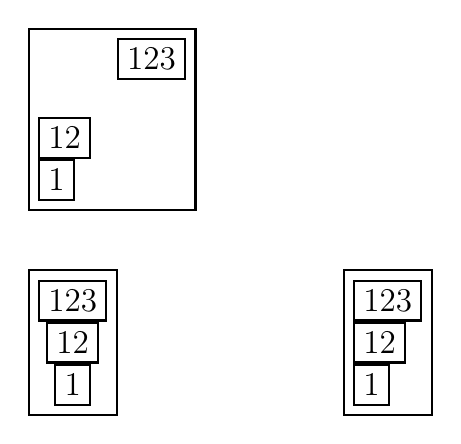
\begin{tikzpicture}

\matrix  [anchor=north west] at (0,1) {
\node at (1,1) {123}; \\ % still center anchor
\node {12}; \\
\node {1}; \\
};

\matrix [matrix anchor=west] at (0,-3) {
\node {123}; \\ % still center anchor
\node {12}; \\
\node {1}; \\
};

\matrix [anchor=west] at (4,-3) {
\node {123}; \\ % inherited west anchor
\node {12}; \\
\node {1}; \\
};
   
\end{tikzpicture}

